\documentclass[russian,utf8, a1paper, emptystyle]{eskdgraph}

\newcommand{\No}{\textnumero} % костыль для фикса ошибки

\ESKDdepartment{Федеральное государственное бюджетное образовательное учреждение высшего профессионального образования}
\ESKDcompany{Московский государственный технический университет им. Н. Э. Баумана}
\ESKDclassCode{23 0102}
\ESKDcolumnI{АИС поиска алгоритмов распознавания изоморфизма графов}
\ESKDcolumnII{Графическая часть}
%\ESKDsignature{Вариант 8Б}
\ESKDauthor{Гуща~А.~В.}
%\ESKDtitleApprovedBy{~}{~\underline{\hspace{2.5cm}}}
%\ESKDtitleAgreedBy{~}{~\underline{\hspace{2.5cm}}}
%\ESKDtitleDesignedBy{Студент группы ИУ5-82}{Гуща~А.~В}
 
\usepackage{multirow}
\usepackage{tabularx}
\usepackage{tabularx,ragged2e}
\renewcommand\tabularxcolumn[1]{>{\Centering}p{#1}}
\newcommand\abs[1]{\left|#1\right|}

\begin{document}

%\ESKDcolumnI{Общие сведения о спроектированной АИС}
\begin{ESKDdrawing}

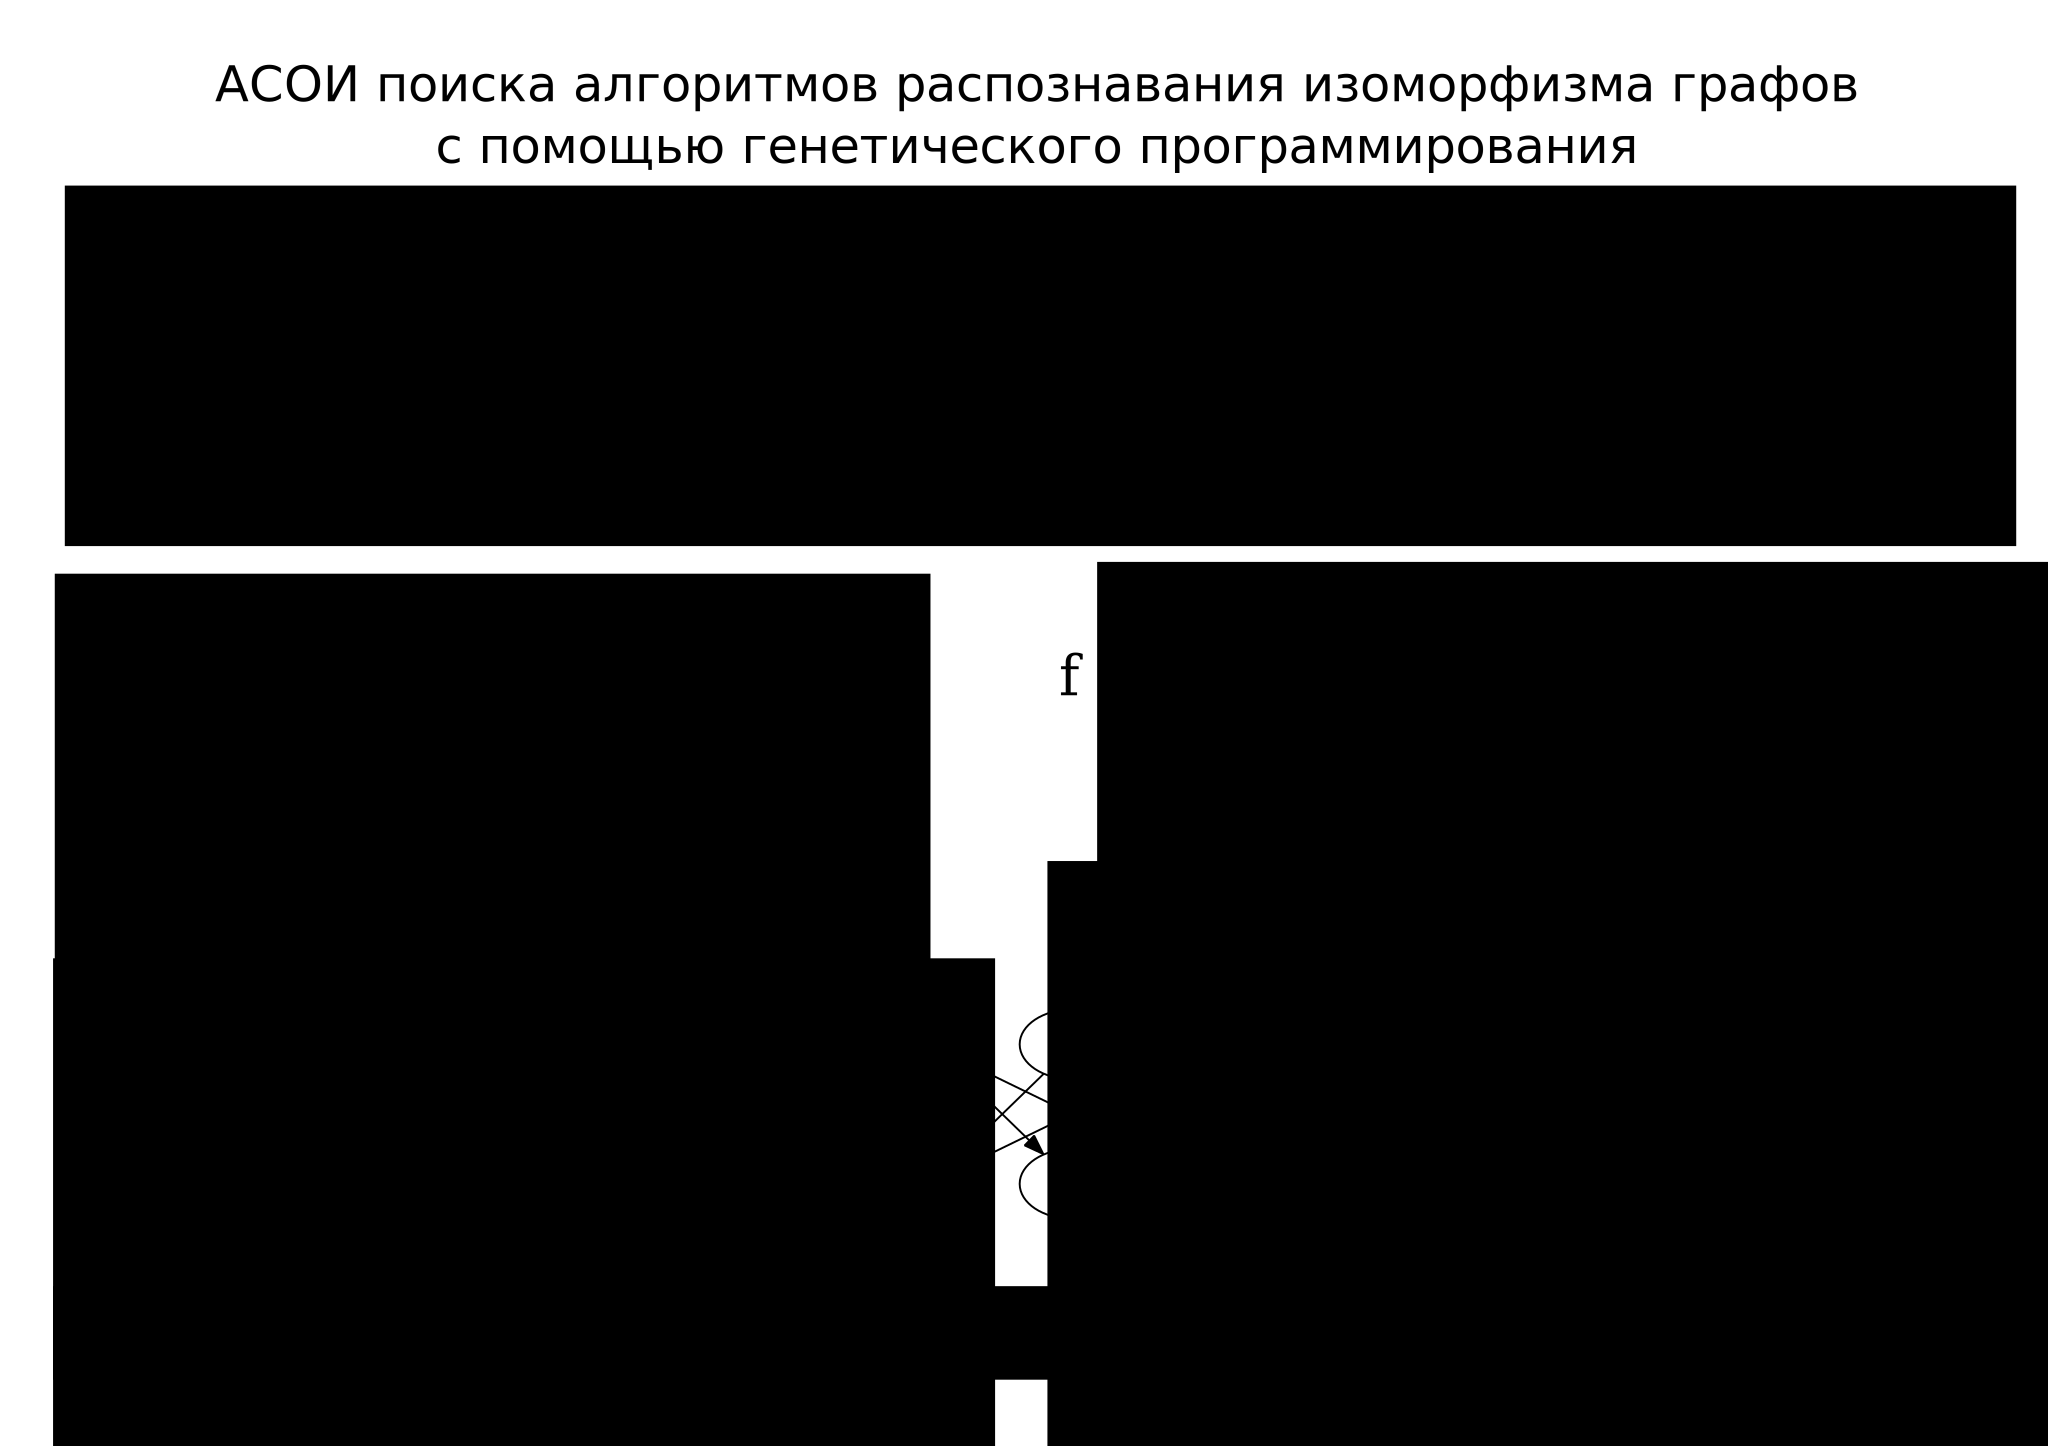
\includegraphics[scale=0.99]{list1}

\end{ESKDdrawing}

%\ESKDcolumnI{Структурная схема АИС}
\begin{ESKDdrawing}
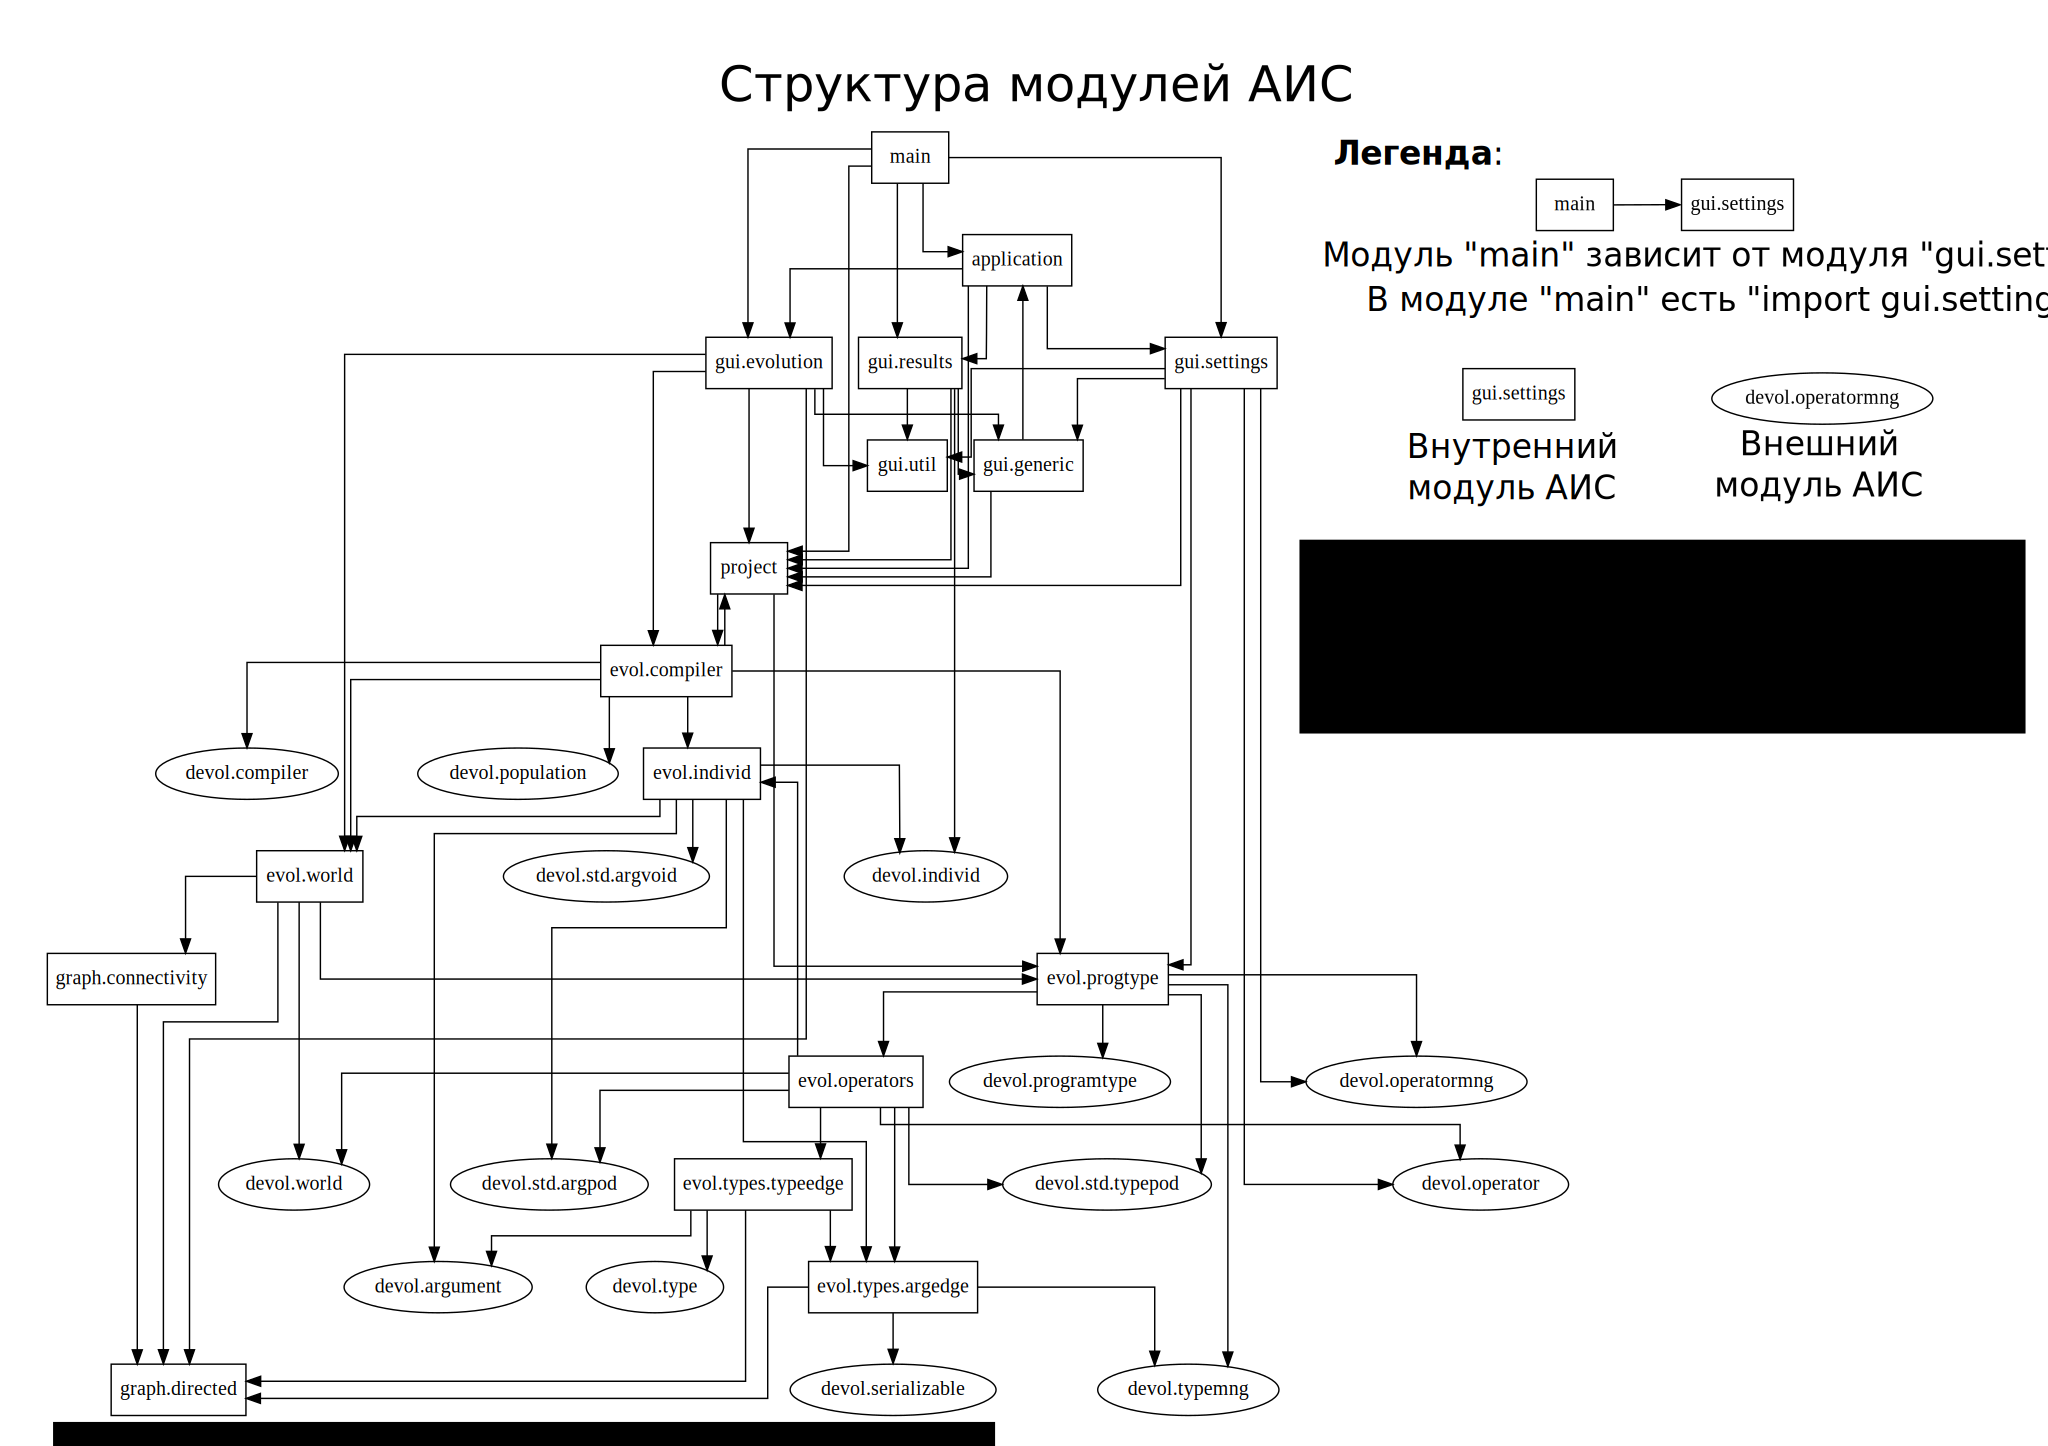
\includegraphics[scale=0.98]{list2}
\end{ESKDdrawing}

%\ESKDcolumnI{Описание DSL генетического программирования}
\begin{ESKDdrawing}
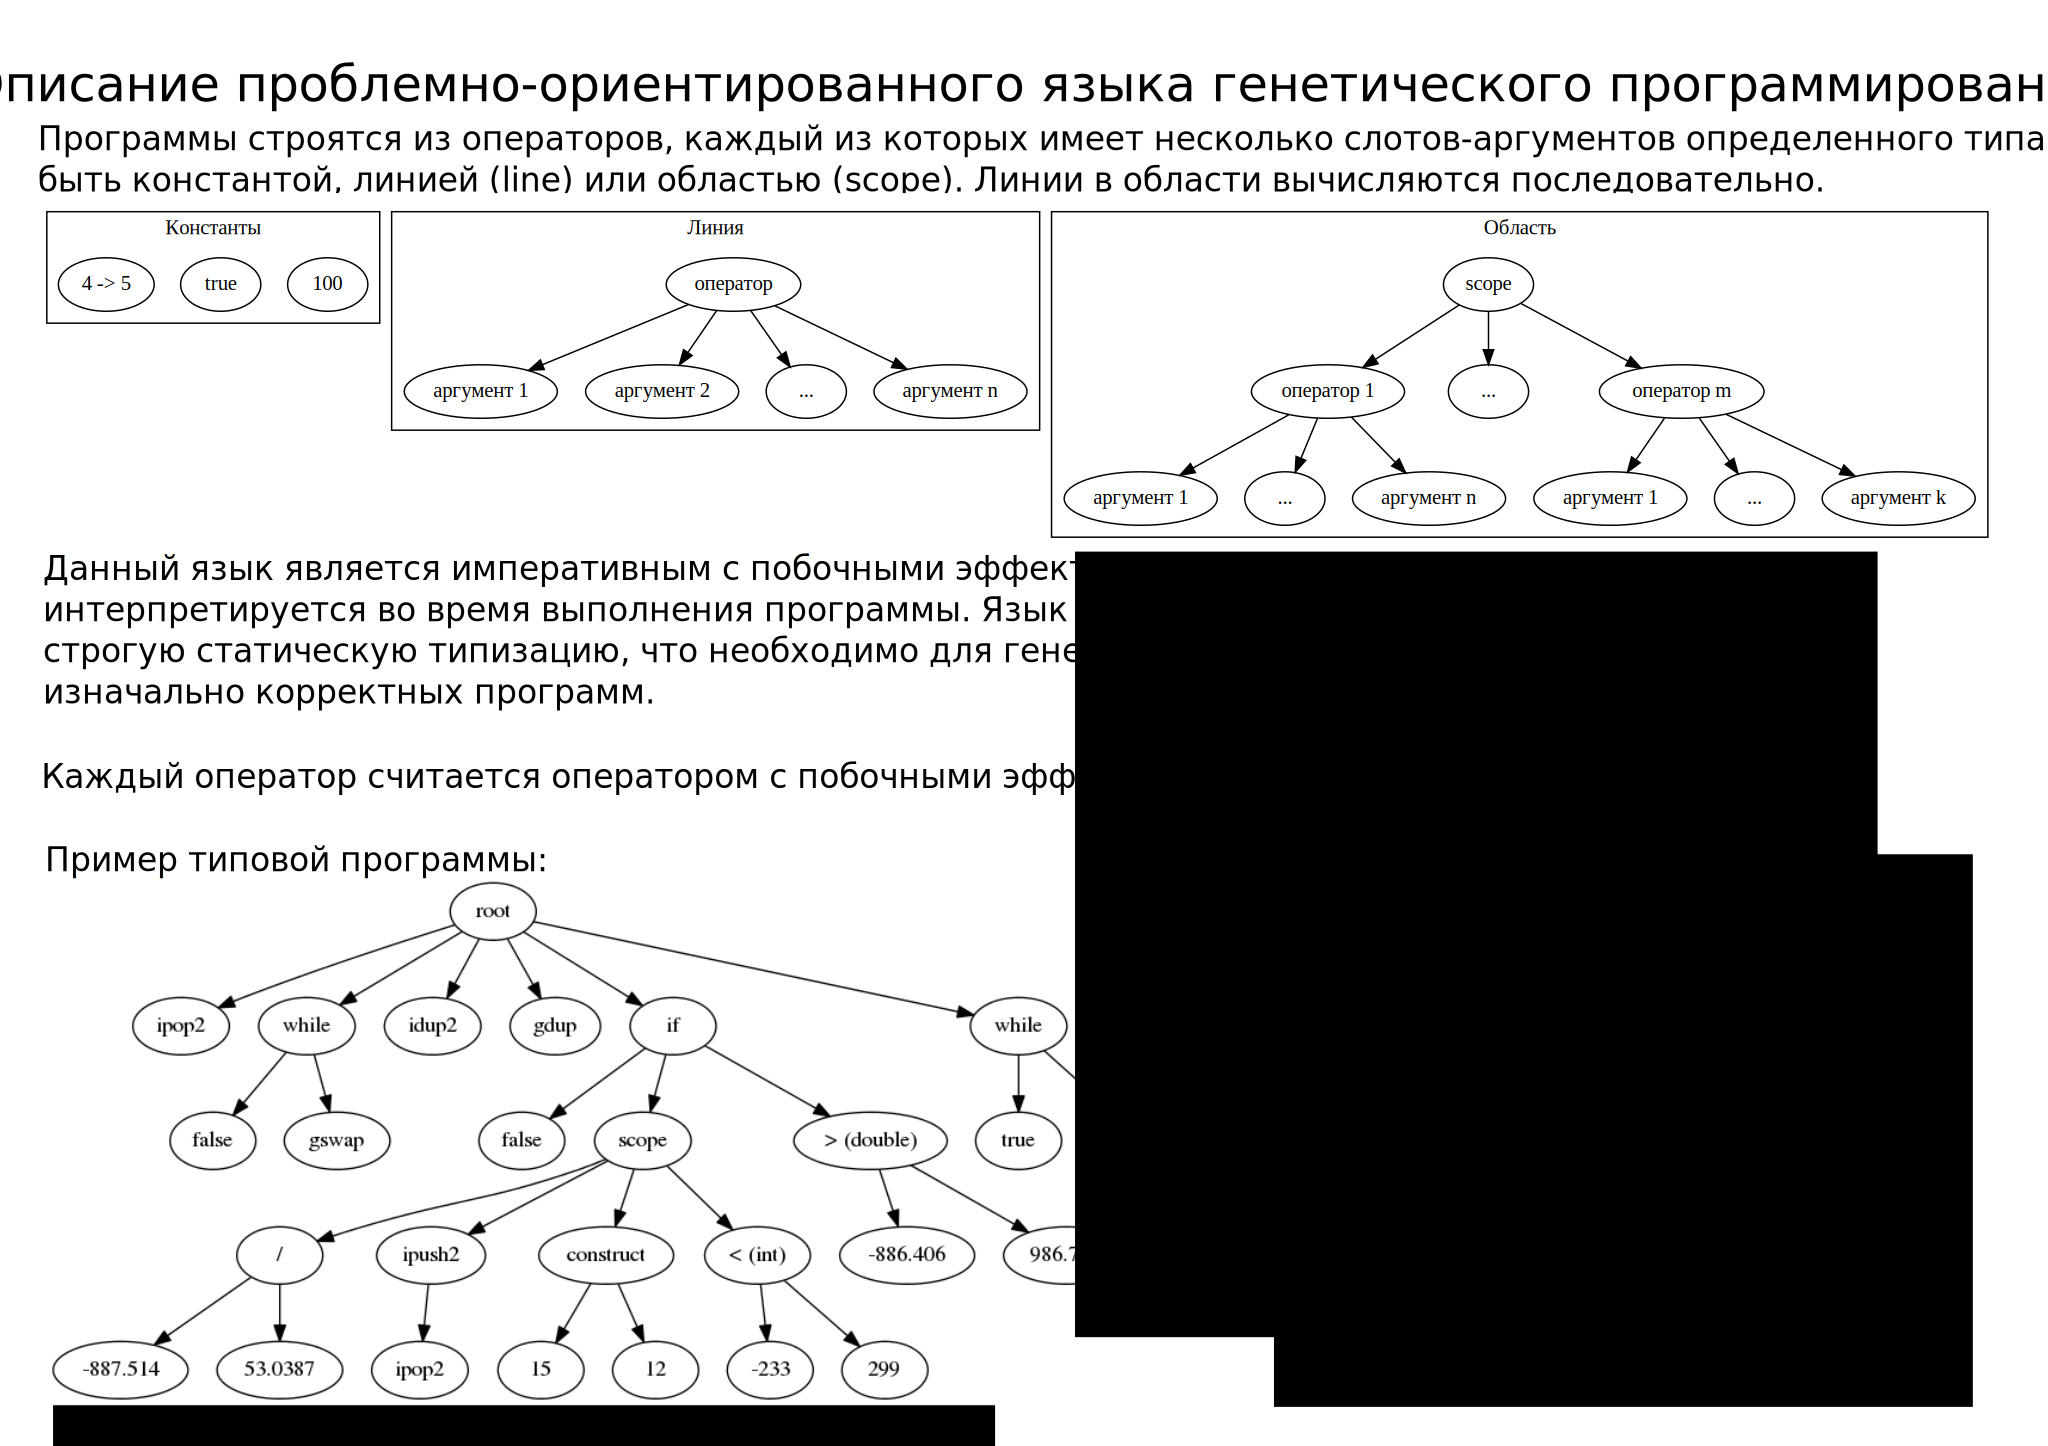
\includegraphics[scale=0.98]{list3}
\end{ESKDdrawing}

\ESKDcolumnI{Основные алгоритмы АИС}
\begin{ESKDdrawing}

\includegraphics[scale=0.99]{list4_1}
\end{ESKDdrawing}

\begin{ESKDdrawing}

\includegraphics[scale=0.99]{list4_2}
\end{ESKDdrawing}

\begin{ESKDdrawing}
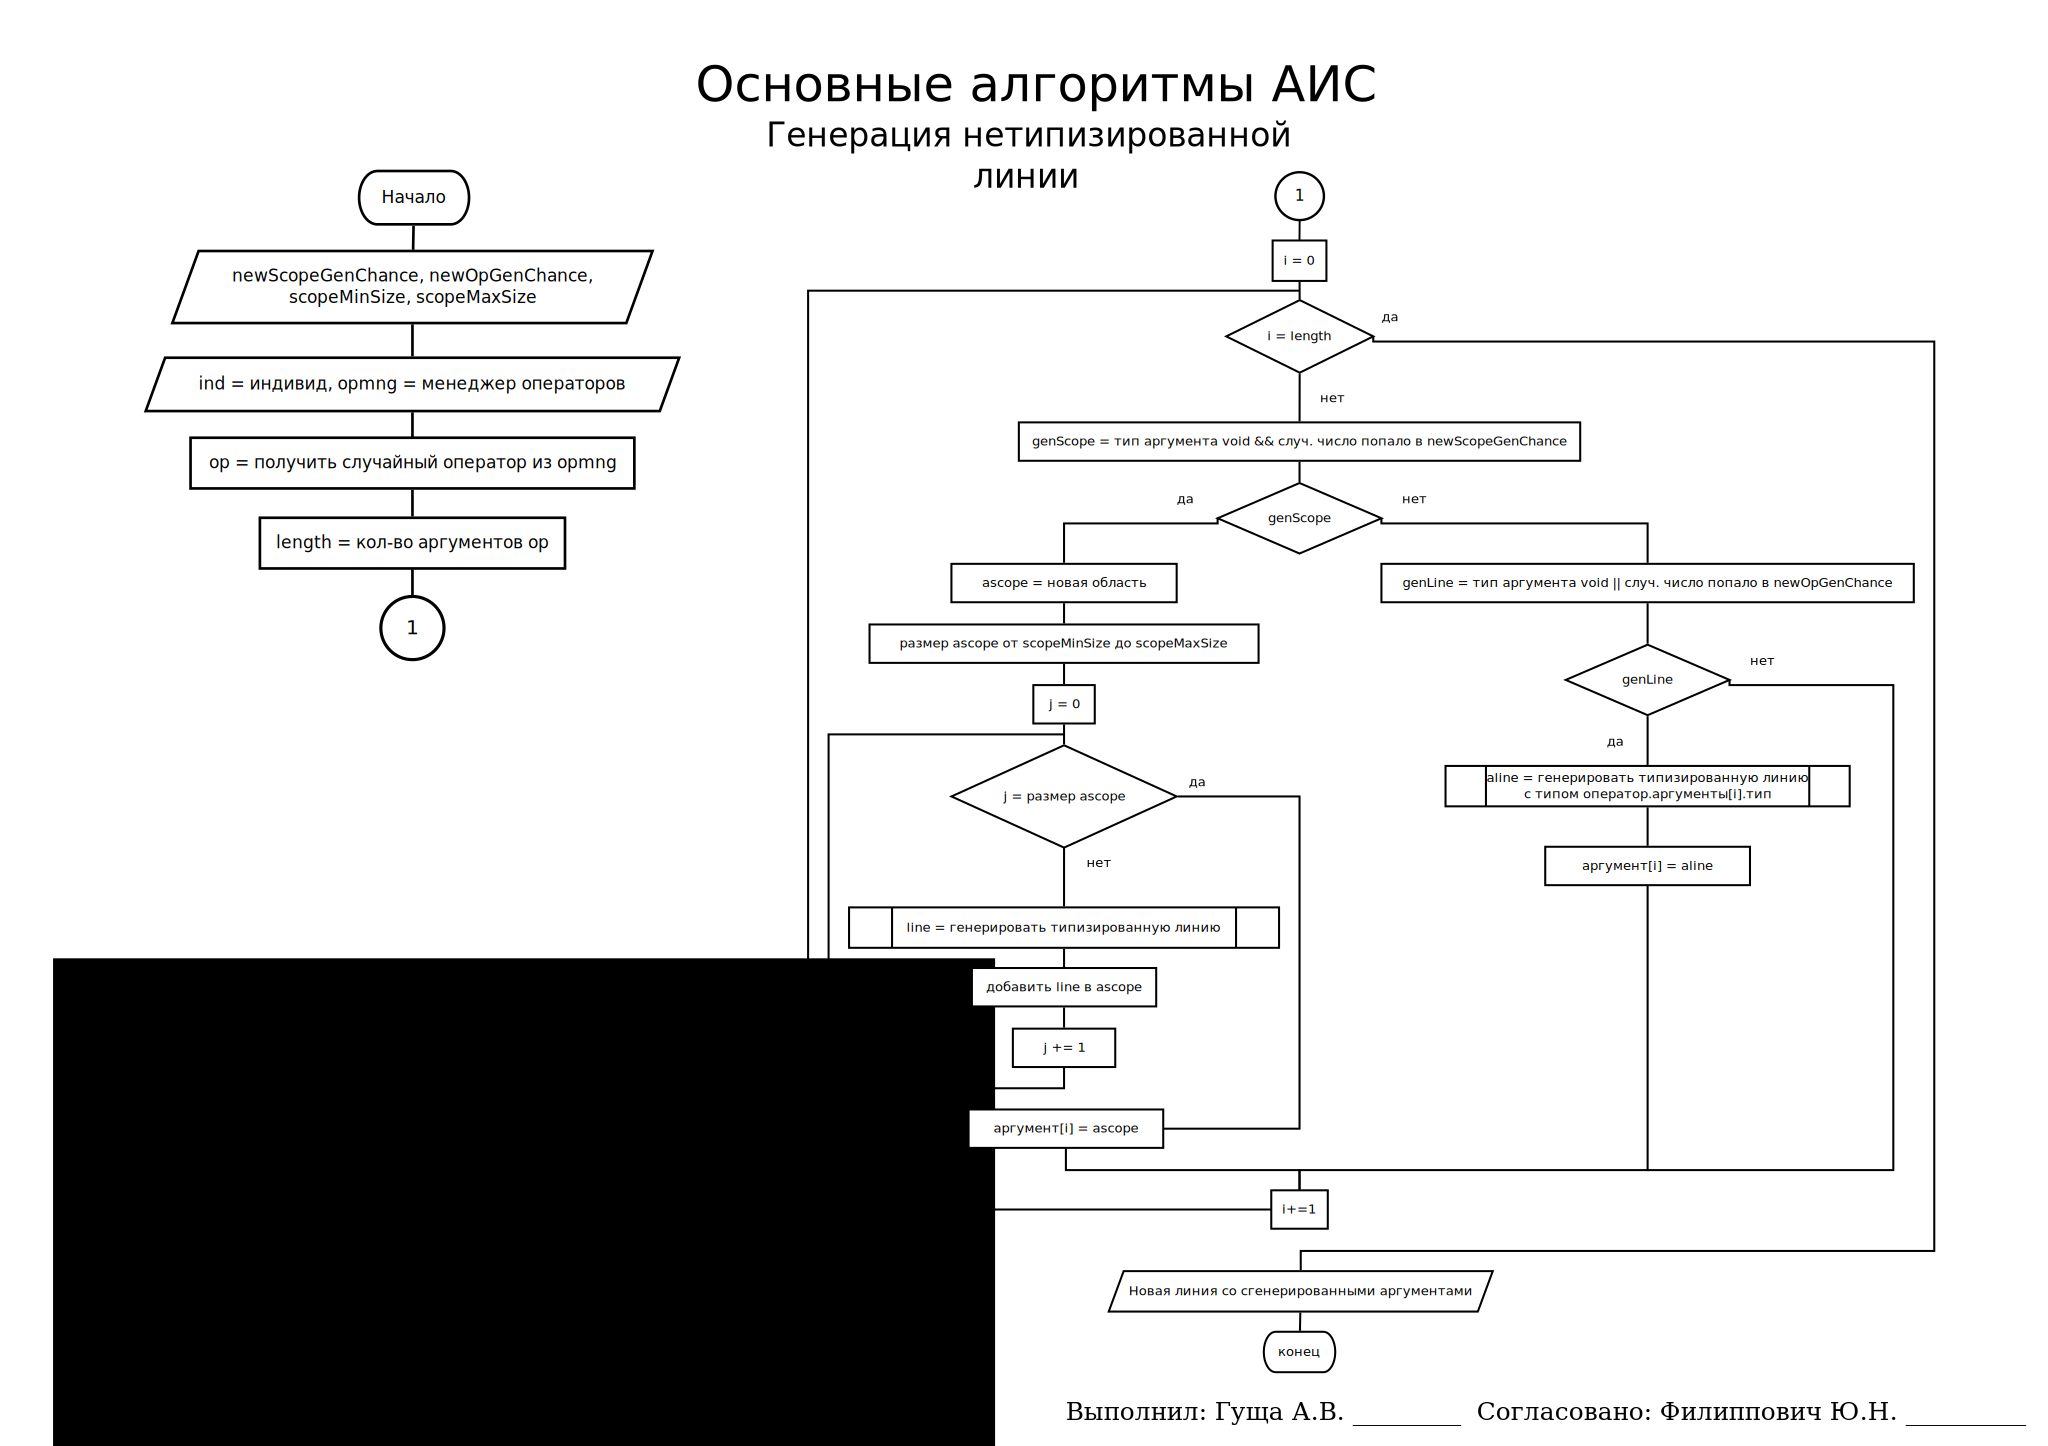
\includegraphics[scale=0.99]{list4_3}
\end{ESKDdrawing}

\ESKDcolumnI{Основные алгоритмы АИС}
\begin{ESKDdrawing}

\includegraphics[scale=0.99]{list5_1}
\end{ESKDdrawing}

\begin{ESKDdrawing}

\includegraphics[scale=0.99]{list5_2}
\end{ESKDdrawing}

\begin{ESKDdrawing}

\includegraphics[scale=0.99]{list5_3}
\end{ESKDdrawing}

%\ESKDcolumnI{Диаграмма классов}
\begin{ESKDdrawing}
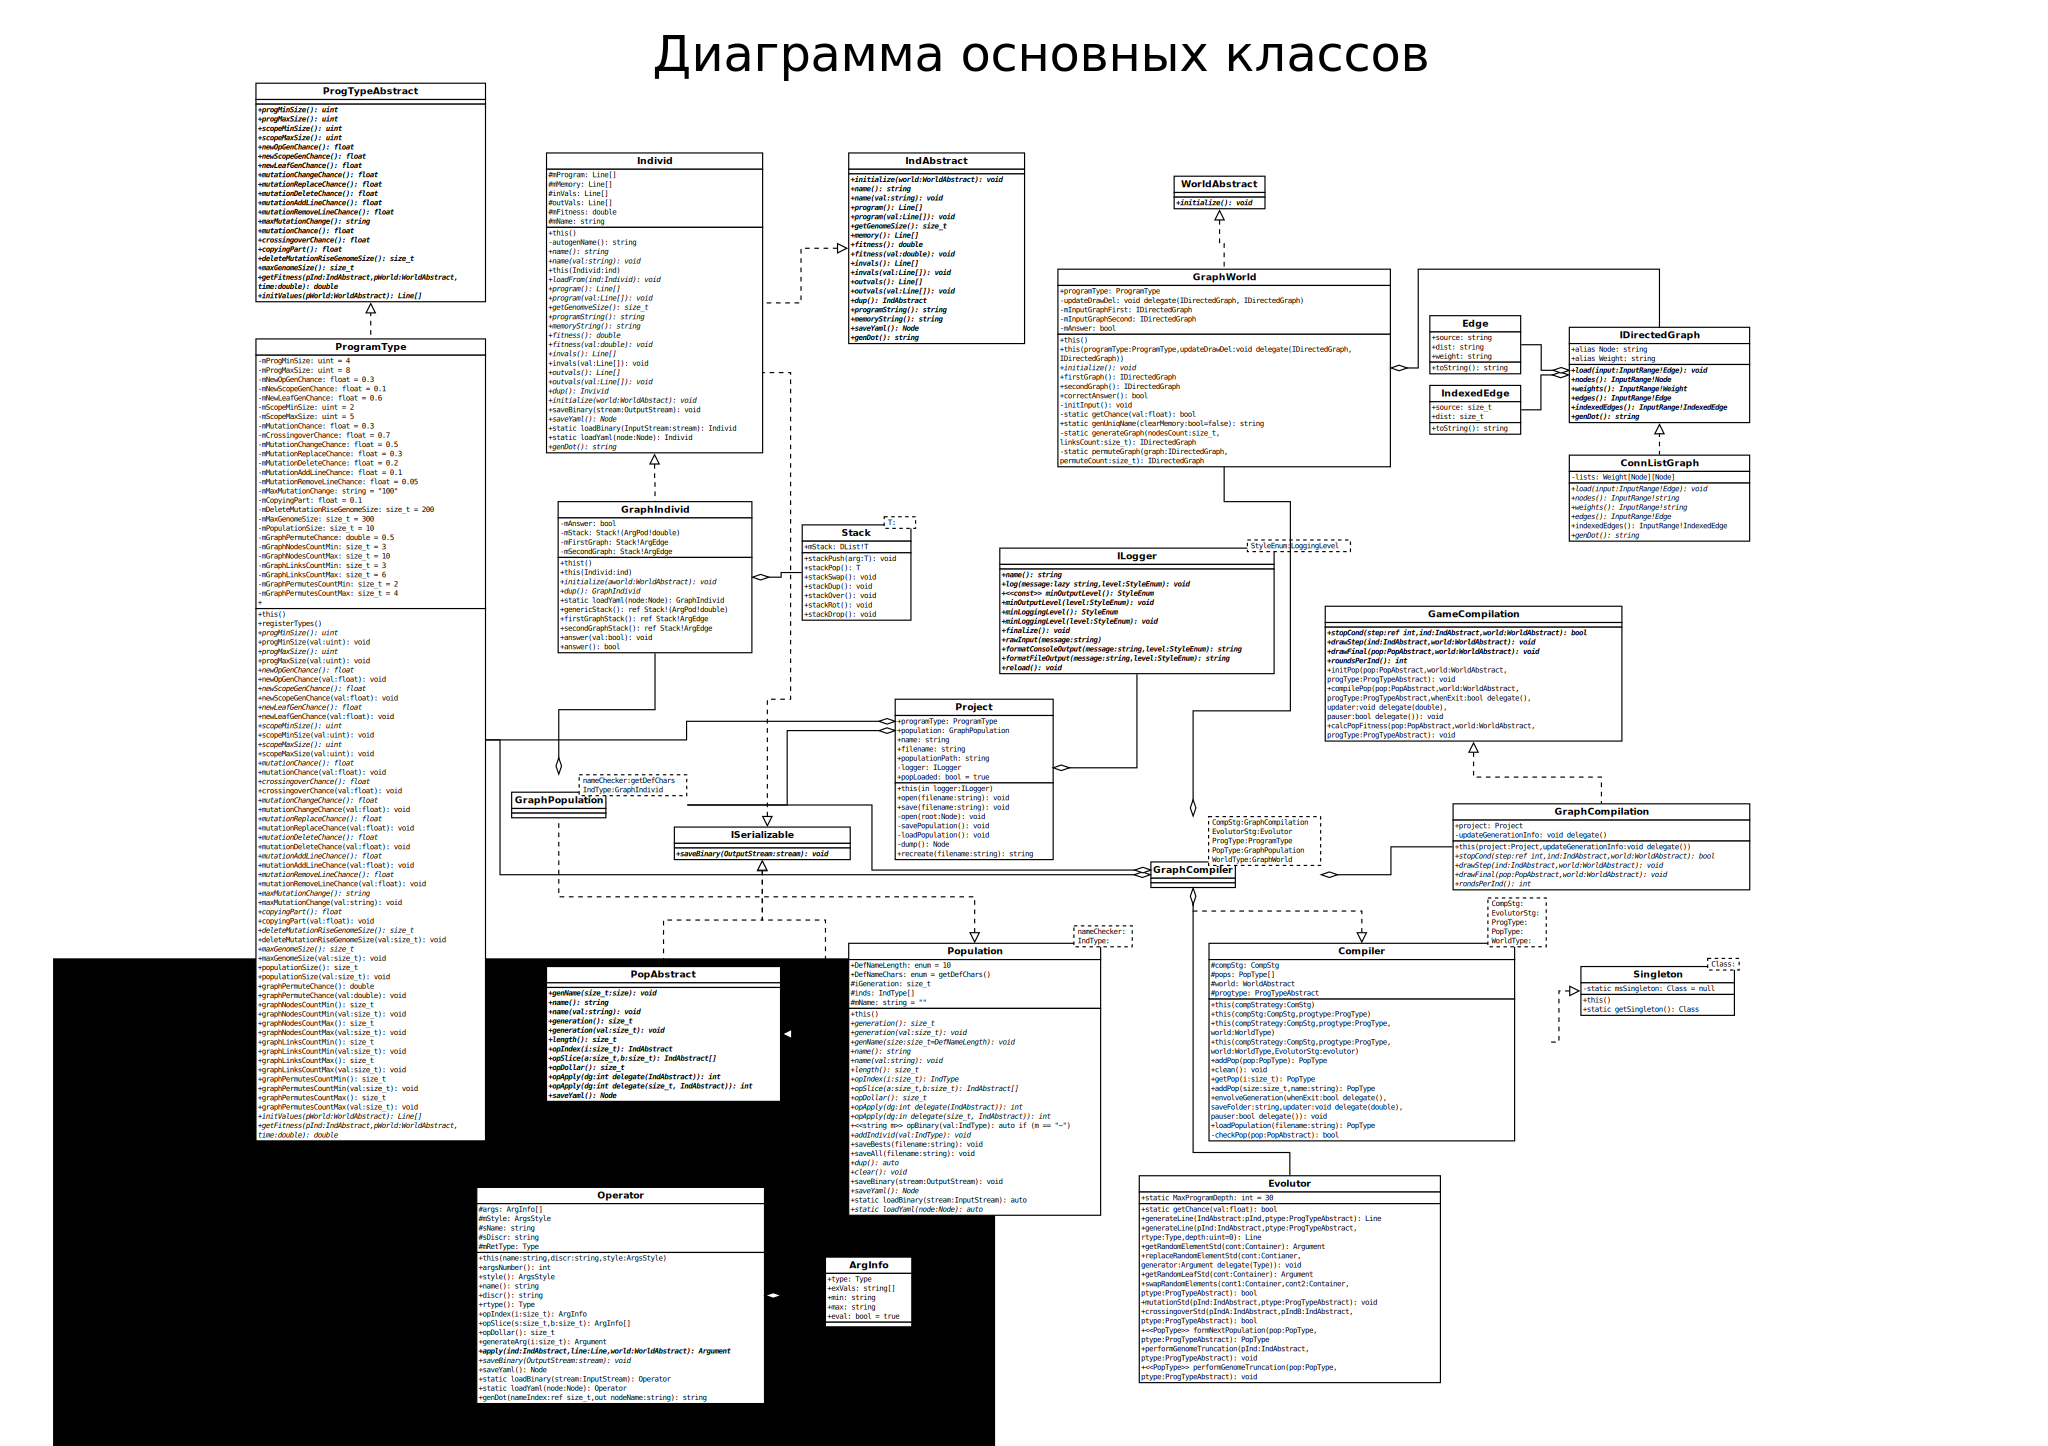
\includegraphics[scale=0.97]{list6}
\end{ESKDdrawing}

%\ESKDcolumnI{Граф диалога с пользователем}
\begin{ESKDdrawing}

\includegraphics[scale=0.98]{list7}
\end{ESKDdrawing}

\end{document}


